\documentclass{puzzlehunt}

\usepackage{tikz-qtree}
\usepackage{amssymb}

\title{Von Braun's Puzzlehunt: Agent Fieldbook}
\author{Escape Pod | Steven Clontz}
\date{\today}

\phSetSquareLogo{escape-pod-logo.png}
\phSetBannerLogo{escape-pod-logo.png}


\begin{document}


\frontmatter % roman page numbers (iv)

\phTitlePage % Print title page.
% \phTableOfContents % Print table of contents


\mainmatter % arabic page numbers (4)


% \phPart{Organizers' Booklet}

\phChapter{From the Desk of J. Edgar Hoover}

\noindent Agents,

A unique situation has arisen in the Huntsville, Alabama area which requires
your services. Our intelligence reveals that several Soviet spies are converging
on Dr. Wernher von Braun's personal office to obtain secret documents vital to
our national security.

We've already sent a team of agents to von Braun's office to find and extract
those classified documents before the Soviets can, but we cannot guarantee
their success. As such, it's up to you to track down the Soviet spies as they
attempt their escape, by following the clues our operatives have uncovered
around the City of Huntsville. You are our last line of defense in this crucial
national security mission, and our fate lies in your hands! Good luck.

- JEH

\begin{center}
  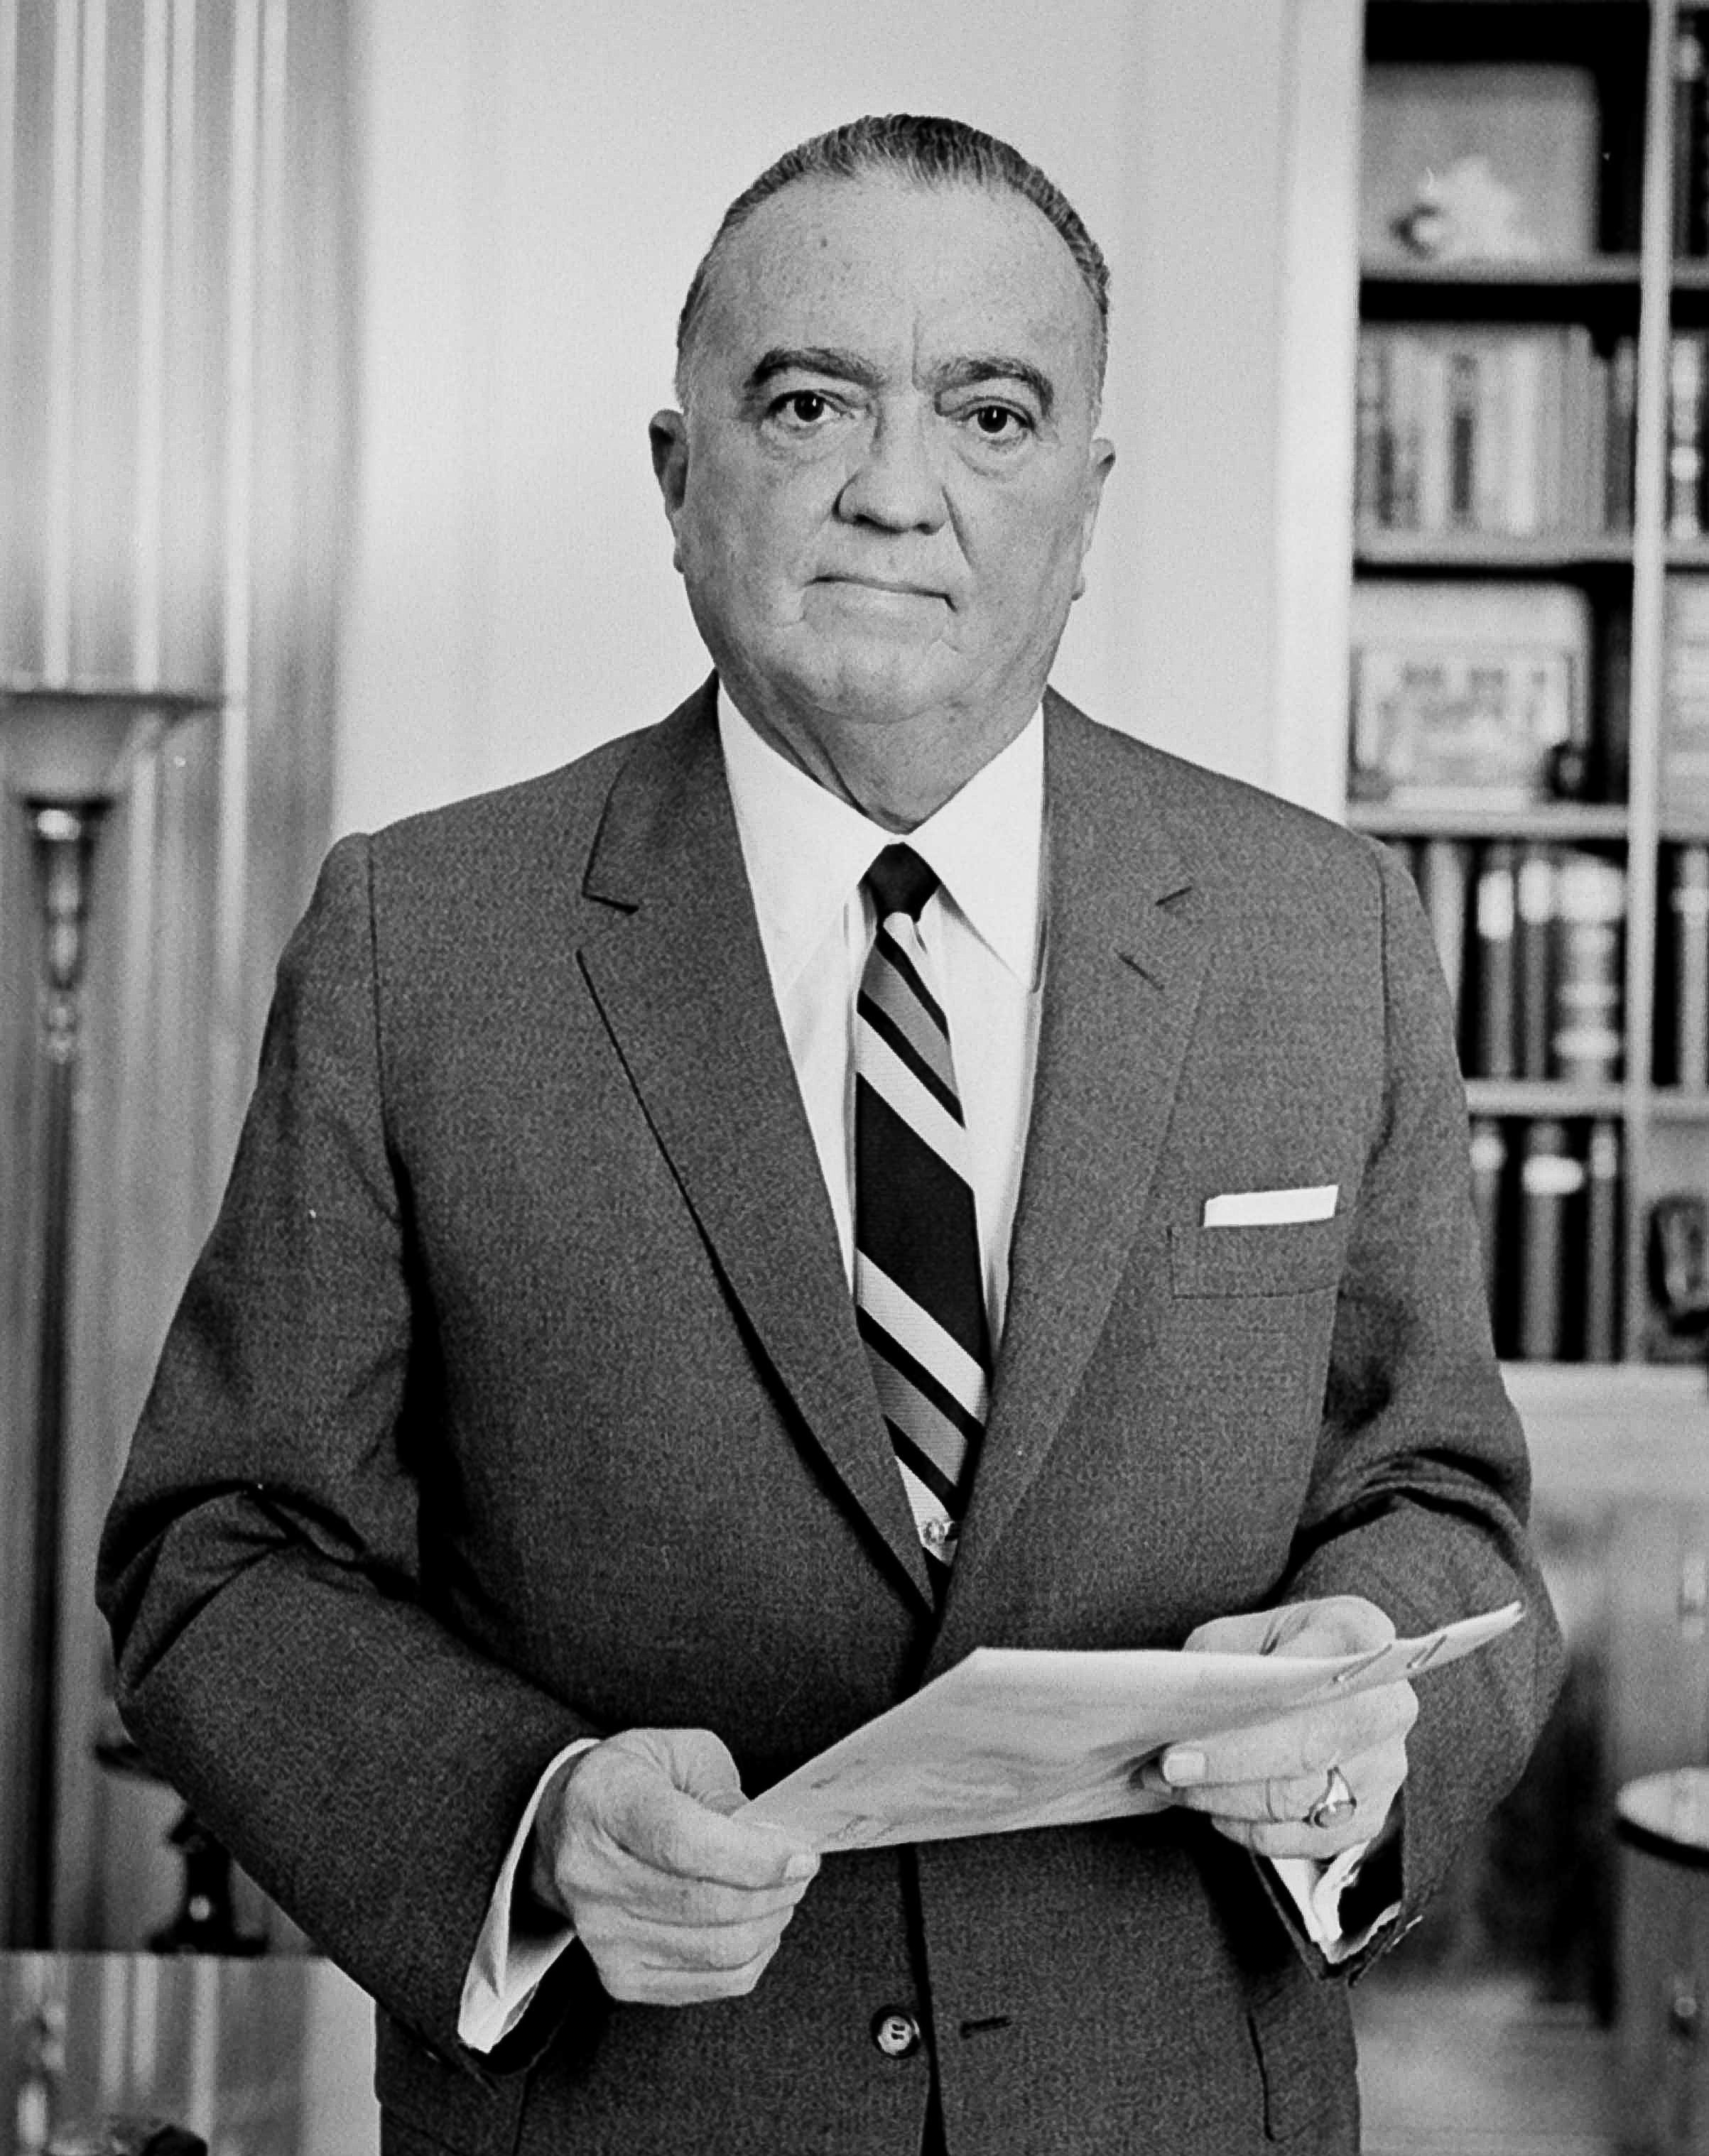
\includegraphics[width=.5\linewidth]{jeh.jpg}
\end{center}

\phChapter{Puzzlehunt Rules}

Welcome to Escape Pod's first \textbf{puzzlehunt} event! A puzzlehunt
is a puzzle-solving competition which takes place throughout an entire city.
You and your team will race between certain locations around Huntsville,
Alabama to discover clues
which will lead to the identity of the fleeing Soviet spies. JEH has a
few prizes for participating teams, so get ready for a fast-paced compeition
against your fellow agents!

Please read these rules, so you'll be prepared for the competition.

\phSection{Time/Date}

The puzzlehunt will be held on \{TODO: date\} beginning at 10am. Teams must
complete the hunt before 3pm to be eligible for prizes.

\phSection{Teams and Registration}

Each participating team must register online at \{TODO: url\} before noon
on the day of the hunt to be eligible for prizes. You must have at least two
players, but otherwise there is no limit to the
number of players on your team. Note that any awarded prizes will be divided amongst
all team members according to the team's registration. We recommend having
a team of between three to five players who can fit in the same vehicle.

You can also play from home or by yourself, but you won't be eligible for prizes, and
it's not quite as much fun.

\phSection{Before the Game}

Your team should download and print the \textit{Agent Fieldbook} (this document!)
for your reference during the competition. It contains important evidence
(read: puzzles) which you'll need to decipher to uncover the identity of the
Soviet spies. Don't bother trying to solve the puzzles before the competition...
they are missing several key components which you'll pick up in the field during
the hunt.

At least one player on your team should have a smartphone (called a
``hand computer'' by the 50s-era characters in the game) with access to the
internet (``ARPAnet''), a camera app, a barcode scanning app, and either
the Facebook (``FB protocol'') or Twitter (``Twttr protocol'') app.
He or she should follow Escape Pod \{TODO: add handles\} and must be able
to post publicly. All posts should include the hashtag \#EscapePodHunt
and a hashtag assigned to your team at registration.

It will be helpful to have a few pencils/pens and notepads as well.

\phSection{Gameplay}

At 10am, Escape Pod will release information via social media which will direct
you to the first \textbf{Location} of the game. At each of the five Locations used
in the game, your team should find a QR code. This will reveal the URL of a
webpage containing a \textbf{Mission Update}.

Most Mission Updates will reveal two things: the key to solving a \textbf{Puzzle},
and a \textbf{Riddle} pointing to your next Location. You may need a page from
this \textit{Fieldbook} to solve the Puzzle, and you may be instructed
to photograph something in the environment to help you as well. The Mission Update
will tell you to upload a photograph to social media, confirming that your team
has visited the Location.

Once you have solved the Riddle and completed any other tasks suggested in
the Mission Update, your team may move on to the next Location. You do NOT have
to solve the Puzzle before moving on; you may wish to work on it while one team member
drives you to the next Location. Please note that all Location clues will refer to
modern Huntsville, despite the game being set in the 50s, so don't overthink it!

Hints will be occassionally distributed via Escape Pod's social media channels
during the game, so you'll want to be following us while you play. If you're playing
from home, we will eventually reveal the Mission Updates and other required information
for working on the puzzles on social media, sometime after teams in the field have
discovered them for themselves.

\phSection{Endgame}

Your final Mission Update will explain how to solve the final
\textbf{Metapuzzle}, which will reveal the identity of the Soviet spies.
You will require the answers to the other Puzzles in order to solve the Meta.
A special webpage will be provided for your team to submit your solution. Your
team is limited to three guesses, so choose carefully! Escape Pod will respond
to submissions via social media. Only submissions before 3pm will be considered.

\phSection{Prizes}

The first team to submit the correct solution on the provided webpage wins the
\textbf{Grand Prize}! \{TODO what is it?\}

All teams that visit all five Locations are considered winners, though, whether
or not they solve all the Puzzles, and will receive a small token recognizing
their acheivement \{TODO what?\}. Another \textbf{Prize} \{TODO what?\} will be
raffled off after the game ends at 3pm. Each team will receive one chance to
win the raffle for completing each of the following tasks:

\begin{itemize}
  \item Posting a public Location photograph to social media.
  \item Posting the \textit{first} public photograph to social media for a Location
  \item Submitting the correct Metapuzzle solution.
\end{itemize}

(Make sure your photos are posted with the correct hashtags so we can find
and count them for the raffle!)

\phSection{Safety and Common Sense}

Have fun, but don't do anything silly. Escape Pod reserves the right to
disqualify any team which does anything unsafe or unfair, and is not liable
for your actions during the game. Keep in mind the following:

\begin{itemize}
  \item Follow all traffic laws when driving. Don't solve and drive; let your
    passengers work on the Puzzles instead.
  \item Don't do anything which prevents other teams from playing or enjoying
    the game, such as moving or removing any QR codes.
  \item Don't jump fences or otherwise trespass on private property. All
    Locations are public areas accessible by driving on roads or walking on
    sidewalks.
  \item Don't do anything which violates the spirit of these rules or the game.
    Contact Escape Pod if there's any question on whether something breaks
    the rules, but if you have to ask...
\end{itemize}

\phSection{Have Fun!}

Contact us at \{TODO contact\} with any questions before the game.

\vfill

{\footnotesize This event was designed by Steven Clontz
\(\langle\)\url{http://clontz.org}\(\rangle\) on behalf of Escape Pod.}


\phChapter{Fieldbook Evidence}

\noindent Agents,

Our operatives have intercepted the following secret messages from the
Soviet spies over the past few weeks. Despite all attempts, we have been
unable to decipher their hidden meanings. We expect that further data
is required to do so.
\textbf{So, you are advised not to attempt to solve these puzzles until you
receive further instructions.} Rather, \textbf{print these pages} and
bring them with you into the field on your upcoming mission.

Don't forget to load either the \textbf{FB or Twttr protocol} on your
\textbf{hand computer} before leaving on your mission. I will be sending
you \textbf{Mission Updates} via those channels during your outing which
will help you decipher these mysterious documents. Be on the lookout for
your first clue on the morning of \{TODO date\}, and good luck!

- JEH


\phWorksheet{Item A}

  VBC von Braun plaque; Scrambled word search

  On website, players get a list of tuples designating the line/word
  which should be found in the scrambled word search. One word is designated
  on the website and on the paper. (These words should be long.)
  The places these words cross is a clue.

  A:

\phWorksheet{Item B}

  Lowe Mill; Skyline puzzles

  The Skyline puzzles are complete, but lack instructions. An answer grid
  is missing most letters; these are filled in using the ``Foundry TVAR''
  sign. The website gives instructions and designates cells to use with the
  answer grid.

\phWorksheet{Item C}

  % Braham Disc Golf; Rock paper scissors logic puzzle
  %
  % Several tournament brackets with seven players are set up, labeled as
  % ``mth word, nth letter''. The website reveals the rules of the logic puzzle
  % to determine how to compute winners in the brackets. The winner of each
  % bracket coresponds to a rule. (``Who rules?'')

  \newcommand{\escapePodTournament}[7]{
    \resizebox{.7\textwidth}{!}{
    \begin{tikzpicture}
      \tikzset{edge from parent/.style=
      {draw,
      edge from parent path={(\tikzparentnode.south)
      -- +(0,-8pt)
      -| (\tikzchildnode)}}}
    \Tree
      [.\(\square\)
        [.\(\square\)
          [.\(\square\)
            #1
            #2
          ]
          [.\(\square\)
            #3
            #4
          ]
        ]
        [.\(\square\)
          [.\(\square\)
            #5
            #6
          ]
          #7
        ]
      ]
    \end{tikzpicture}
    }
  }

  \begin{center}
    \escapePodTournament{1}{2}{3}{4}{5}{6}{7}
  \end{center}

  \begin{center}
    \escapePodTournament{1}{2}{3}{4}{5}{6}{7}
  \end{center}

  \begin{center}
    \escapePodTournament{1}{2}{3}{4}{5}{6}{7}
  \end{center}

  \begin{center}
    \escapePodTournament{1}{2}{3}{4}{5}{6}{7}
  \end{center}

  \begin{center}
    \escapePodTournament{1}{2}{3}{4}{5}{6}{7}
  \end{center}

\phWorksheet{Item D}

  Joe Davis Stadium; Braille code criss-cross

  Words related to Military (ACTIVE, DUTY, RESERVE, NATIONAL, GUARD,
  RETIREE, FAMILY, MEMBERS, VETERANS) are converted to Braille and
  put into a criss cross.

\phWorksheet{Item E}

  % \vfill
  %
  % \begin{center}
  %   \begin{tikzpicture}[x=1.7cm,y=1.7cm]\LARGE
  %     \node at (1,3)
  %       {Abram};
  %     \node at (3,3)
  %       {Anton};
  %     \node at (5,3)
  %       {Artur};
  %     \node at (7,3)
  %       {Bagda};
  %     \node at (1,2)
  %       {Boris};
  %     \node at (3,2)
  %       {Denis};
  %     \node at (5,2)
  %       {Fedor};
  %     \node at (7,2)
  %       {Ignat};
  %     \node at (1,1)
  %       {Makar};
  %     \node at (3,1)
  %       {Motya};
  %     \node at (5,1)
  %       {Oskar};
  %     \node at (7,1)
  %       {Pavel};
  %     \node at (1,0)
  %       {Pyotr};
  %     \node at (3,0)
  %       {Timur};
  %     \node at (5,0)
  %       {Yakov};
  %     \node at (7,0)
  %       {Yegor};
  %   \end{tikzpicture}
  % \end{center}

  \vfill

  \newcommand{\escapePodHuntMetaGrid}{
    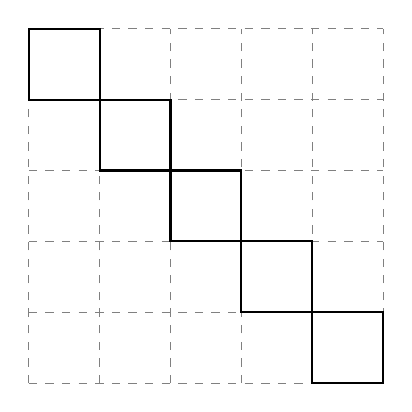
\begin{tikzpicture}[x=0.9cm,y=0.9cm]\Large
      \draw[step=0.9cm, gray, dashed] (0,0) grid (5,5);
      \foreach \x in {0,...,4}
        \draw[thick] (\x,5-\x) rectangle (\x+1,4-\x);
    \end{tikzpicture}
  }

  \phSection{Who are the three Soviet spies?}

  \hspace*{\fill}
  \escapePodHuntMetaGrid
  \hspace*{\fill}
  \escapePodHuntMetaGrid
  \hspace*{\fill}
  \escapePodHuntMetaGrid
  \hspace*{\fill}

  \vfill
  \vfill

  % Codewords:
  % AtOmS
  % oNaIR
  % BeTTy
  % POlOs
  % bYRoN
  %
  % Solution:
  % Anton
  % Boris
  % Pyotr



\end{document}
